
\documentclass{sig-alternate}
\usepackage{color}
\usepackage[colorinlistoftodos]{todonotes}
%\usepackage{float}


%%%%% Uncomment the following line and comment out the previous one
%%%%% to remove all comments
%%%%% NOTE: comments still occupy a line even if invisible;
%%%%% Don't write them as a separate paragraph
%\newcommand{\mycomment}[1]{}

\begin{document}

% --- Author Metadata here ---
\conferenceinfo{UMM CSci Senior Seminar Conference, April 2016}{Morris, MN}

\title{Security of Near Field Communication:\break Does My Phone Need A Tinfoil Hat?}

\numberofauthors{1}

\author{
\alignauthor
Thomas Harren\\
	\affaddr{Division of Science and Mathematics}\\
	\affaddr{University of Minnesota, Morris}\\
	\affaddr{Morris, Minnesota, USA 56267}\\
	\email{harre096@morris.umn.edu}
}

\maketitle
\begin{abstract}
Near Field Communication is a technology that is rapidly growing in popularity and is becoming even more accessible due to the advent of mobile payment systems. \textit{Near Field Communication} (NFC) is built upon High Frequency Radio Frequency Identification technology, more commonly known as HF RFID. However, NFC is a richer communication method: it supports both passive and active components, but at a shorter range. Uses of NFC technologies are being rapidly developed to be used in payment systems and for other applications. 

NFC is a flexible communication technology, but it is not inherently secure. The limited range of NFC offers some security, but data transmitted using NFC is still vulnerable to various attacks. As a result, measures to ensure confidentiality, integrity, or authentication need to implemented as an extension of NFC. Moreover, if the data transmitted from a peer is malicious, a hardware-based firewall may be a good way to defend your NFC capable device. One proposed technology is a device-independent security method, a metaphorical tin foil hat, that could offer flexibly against current and evolving attacks on NFC enabled devices.
\end{abstract}

\keywords{Near Field Communication, Payments, Security}

\section{Introduction}
\label{sec:introduction}
Near Field Communication is a technology that is rapidly growing in popularity and is becoming even more accessible due to the advent of mobile payment systems. \textit{Near Field Communication} (NFC) is built upon High Frequency Radio Frequency Identification technology, more commonly known as HF RFID. NFC is restricted to a shorter range than RFID and offers interactive communication method between devices that have both passive and active components. An NFC connection can be set up quickly and connectivity does not require line of sight. Uses of NFC technologies are being rapidly developed to be used in payment systems and in other applications~\cite{Gum2013}. 

NFC is a flexible communication technology, but it is not inherently secure. The limited range of NFC offers some security, but data transmitted using NFC is still vulnerable to various attacks. For sensitive data, measures to ensure confidentiality, integrity, or authentication need to implemented as an extension of NFC~\cite{CC2016}. In addition, there is no protection against other parties that may have malicious intent. One proposed technology offers a flexible hardware firewall may be an effective way to block data transfers with malicious peers~\cite{Gum2013}.

In this paper, we focus on security and applications of NFC regarding payments and ticketing. First, we describe the foundations of Near Field Communication and the mobile payment ecosystem in Section~\ref{sec:background}. After the background section, we discuss security in three different NFC contexts: contactless credit cards, mobile ticketing applications, and physical NFC security. 
We highlight a recent academic source that describes issues and proposes a solution for NFC security in the context of contactless credit cards in Section~\ref{sec:creditCard}. 
In Section~\ref{sec:mobile}, we discuss a prospective application for the richer NFC communication offered when using mobile phones. In particular, this section focuses on  using mobile phones for mass transit ticketing. Three implementations of mobile ticketing, each balancing security and transaction time in a unique way, are introduced, prototyped, and critiqued.
This leads to a discussion about the EnGarde shield in Section~\ref{sec:enGarde}. Commercial payment systems such as Apple Pay and Android Pay are bringing NFC to mobile phones, which could introduce security risks in both payment and non-payment applications of NFC. The proposed device independent, hardware-based firewall may be a viable way to defend against more general threats. \textcolor{red}{Finally, we to preview some developing applications and summarize the state of security on the NFC platform.}


%%%%%%%%%%%%%%%%%%%%%%%%%%%%%%%%%%%%%%%%%%%%%%%%%%%%%%%%%%%%%%%%
\section{Background}
\label{sec:background}
In this section, we provide an overview of Near Field Communication and properties of its physical operation.  We first discuss RFID technology, the parent technology of NFC. Next, we discuss additional features specific to the NFC standard. Since this paper emphasizes NFC in the context of payments, we will briefly describe the current status of the payment industry. \textcolor{red}{Finally, we introduce common security protocols that could possibly be a means of securing NFC.}

\subsection{Elements of HF RFID: Tags \& Readers}
\label{sec:activePassive}

NFC is a wireless communication standard that is based on, and fully compatible with, the HF RFID (high frequency radio-frequency identification) standard.~\cite{Gum2013} At a fundamental level, this means that communication happens between tags and readers. 

A \textit{tag} is composed of an integrated circuit and an antenna. A tag is capable of storing a unique ID and a limited amount of data, which can be read/write or read only. RFID tags can be actively powered, battery assisted, or passively powered. A passive tag relies exclusively on energy induced into the tag's antenna coil. Since passive tags require no built in power source, they are the least expensive and smallest RFID tags. While the tag is powered, it can use its antenna coil to relay its internal information back to the asking party.~\cite{wiki:RFID}

A \textit{reader} is a device used to power and interrogate RFID tags. A reader emits an electromagnetic field in order to power nearby tags. Before initiating communication, the reader runs a discovery protocol. If multiple tags respond, the reader uses its collision avoidance protocol to establish communication with a single tag using one tag's unique ID. The tag and the reader then communicate by taking turns sending and receiving messages.~\cite{Gum2013}

A standard RFID reader-tag interaction is illustrated in Figure~\ref{fig:rfid}. Both the reader and tag have antenna coils tuned to 13.56MHz. When the reader generates an electromagnetic field, the reader and the tag are coupled, and power is induced into the tag's antenna coil; this energy transfer is similar to that found in electrical transformers. The tag then converts the AC voltage it receives into DC voltage in order to power the tag's circuit. The electromagnetic field of this frequency is able to power a tag within a range of a few centimeters. According to Gummeson et al, the communication distance can be increased up to 1 meter if larger, higher powered readers are used.~\cite{Gum2013}


%\textcolor{red}{Communication happens using amplitude modulation (AM) from the reader to the tag. Then the tag uses a parallel resistor to modulate the load across the tag coil. Varying the load leads to varying the current and voltage that the reader coil receives. Various encoding schemes are then used to send messages in this way.} 
\begin{figure}
\centering
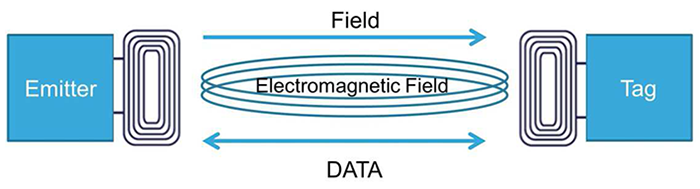
\psfig{file=figures/emitterAndTag.png,width=3in,natwidth=700,natheight=189}
\caption{Readers and tags interact with each other using tuned antenna coils and electromagnetic induction. \todo[inline]{Create custom version and remove citation}
\cite{emmiterAndTag}}
%Neat diagram from http://www.mouser.com/applications/rfid-nfc-introduction/ and another at http://electronicdesign.com/communications/nfcrfid-ripe-application-expansion
\label{fig:rfid}
\end{figure}

\subsection{NFC on Mobile Phones}
\label{sec:nfcOnPhones}
Near field communication also has features that extend beyond the HF RFID specification. In particular, NFC enabled mobile phone can function in several unique modes:
\vspace{2mm}\newline
\textbf{Phone acting as a reader:}
In this mode, a mobile phone functions as an RFID tag reader. Touching a phone to a tag mounted to a map, for example, could send the phone a hyperlink to a informational page.~\cite{staticDynamicDisplays} 
\vspace{2mm}\newline
\textbf{Phone emulating a tag:}
A mobile phone can also function as if it was a passive tag. This mode can be effectively used even when the phone is not powered, because power is induced by an NFC reader. Mobile payments and other ticketing applications would tend toward this interaction mode.~\cite{Gum2013}
\vspace{2mm}\newline
\textbf{Phone acting as a peer:}
When two compatible devices are capable of switching between reader and tag emulation mode, they can communicate directly over NFC in a peer-to-peer manner. Peer-to-peer mode offers the highest communication throughput and can be used to implement stronger security~\cite{Ticket2011} or to coordinate mobile file transfers.~\cite{Gum2013}

\subsection{NFC and the Payment Industry}
\label{sec:paymentIndustry}
Since this paper emphasizes NFC in the context of payments, we will briefly describe the current status of the payment industry.
\vspace{2mm}\newline
\textbf{EMV:}
EVM is a global standard, developed by Europay, MasterCard, and Visa, that defines chip-based credit card standards as well as three offline data authentication techniques.~\cite{Ticket2011} EMV chip technology is an alternative to magnetic stripe based cards. Apple Pay and Android Pay are built on top of  
\textcolor{blue}{Based on questions I have received, I think it is critical that better explain the current state of payments in a more general sense. However, most of the stuff about EMV and Apple Pay is industry developed and thus not covered well in research as far as I can tell. This is an issue since I would ideally like to talk about some of these technologies more extensively, but it only further restricts the space in which I can cover \textit{three} other sources...\newline
The first source I use was published in 2016, but I am not sure that it is relevant without an explanation. I have not yet found an academic source for this, but my conclusion is that the insecure credit card protocol described in Section ~\ref{fig:currentCC} and been mostly, if not totally discontinued. However there is no clear statement of why this happened, but I would bet that it was due to the exact security concerns mentioned. Still, the source does point out that the "near" in NFC does not guarantee security.\newline
Starting about this year, EMV (Europay-Visa-MasterCard) chip and pin have caught on big in the states. I think this may be in part a response to the glaring security risks of sticking with magnetic strips. This is an important discussion as well, because without it most folks have no idea where NFC fits into the industry. \newline
The crucial next step would be to explain that Apple Pay and Android Pay are wireless implementations of the EMV standard. And that other things beyond payments are being developed to take advantage of NFC technology. Then, I think people will be semi-comfortable with background.}~\cite{wired}

\subsection{Security for NFC}
\label{sec:backgroundSecurity}
NFC is a flexible communication technology, but it is not inherently secure. The limited range of NFC offers some security, but data transmitted using NFC is still vulnerable to several attacks. As a result, measures to ensure confidentiality, integrity, or authentication need to implemented as an extension of NFC.~\cite{CC2016}
\vspace{2mm}\newline
\noindent\textbf{Trusted Hardware:}
Mobile phones are capable of doing cryptographic operations which are executed in the phone's \textit{trusted execution environment}, or TEE. Several types of TEEs have been developed in the last decade and are now widely deployed on phones. Some TEEs are hardware agnostic while others extend core processing to strengthen security.
~\cite{Ticket2011}  
\vspace{2mm}\newline
\textbf{Secure Communications:}
There are various methods for securing communication over an insecure channel such as NFC. In a simple symmetric key system, both parties have a secret key that is used to encrypt and decrypt messages at each end of a communication channel. This works very well, but distributing the private key to both parties can present a problem. The public key system works differently than this, requiring a both a private key and a complementary public key. Public keys are distributed and can be used by anyone to encrypt a message that can only be decrypted by the matching private key.~\cite{crypto}




%%%%%%%%%%%%%%%%%%%%%%%%%%%%%%%%%%%%%%%%%%%%%%%%%%%%%%%%%%%%%%%%
\section{Contactless Credit Cards}
\label{sec:creditCard}
In this section, we look at the usage of passively powered NFC tags installed into the  credit cards and some related security concerns. Jensen, Gouda, and Qiu describe several effective contactless credit cards attacks and propose a security protocol to defend against these attacks. Since their security protocol must run on a passively powered NFC chips embedded in credit card, it is composed of computational inexpensive primitives including pre-computed hashes, indexing and XOR operations.~\cite{CC2016}


\subsection{Current Credit Card Protocol}
\label{sec:currentCC}
As background, we will describe the current credit card protocol used for NFC transactions. The current protocol does offer some level of security by merit of the iCVV. A dynamic card verification value or \textit{iCVV} is single use value that a contactless credit card generates each transaction~\cite{wiki:iCVV}. The iCVV is actually returned from a pesudo-random sequence using a seed known only to that specific credit card and the issuing bank. At the time of authorization, the bank checks that the iCVV received is one the expected values in that card's iCVV sequence. The four phases of the credit card protocol used for NFC transactions, are illustrated in Figure~\ref{fig:currentCC}, and will now be described.

In the first phase, called \textit{solicitation}, the point-of-sale and the credit card exchange several messages in a static manner. In this phase, each both parties share general information about themselves. For example, a card may identify itself as \texttt{VISA CREDIT}.

In the second phase, \textit{card information} is sent from the card to the point-of-sale. The card information is composed of the credit card number, the credit card's expiration date, the iCVV, and the name of the bank that issued the card.

The point-of-sale then sends the card information to the bank in the third phase, called the \textit{charge request}. The credit card's number and expiration date, along with the iCVV and the dollar amount charged, are sent to the specified bank.

The final phase is called \textit{authorization} and only occurs if the bank deems the card information valid. Banks may also perform other checks based on the transactions physical location or other factors.


\begin{figure}
\centering
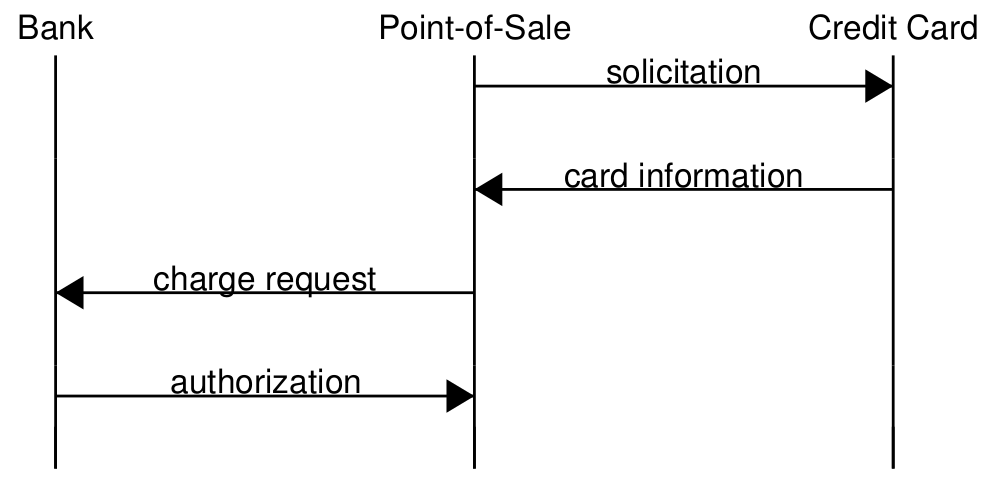
\psfig{file=figures/currentCC.png,width=3in,natwidth=700,natheight=189}
\caption{The basic steps executed in an NFC transaction using the current credit card protocol.
\cite{CC2016}}
\label{fig:currentCC}
\end{figure}

\subsection{Credit Card Attacks}
\label{sec:attacks}
The following attacks on NFC transactions may vary slightly in agency, but each method ultimately exposes sensitive card information. The first three attacks can be accomplished with merely a NFC compatible mobile phone and some additional, inexpensive hardware. The final attack, compromised point-of-sale, points out a more general weakness about the implementation of the current protocol.
\vspace{2mm}\newline
\noindent\textbf{Eavesdropping:}
In this attack, a malicious party is able to capture sensitive data by listening in on the first two phases of an NFC transaction. Thus, the card number, expiration data, iCVV, and bank name are gleaned by the malicious party. The iCVV cannot be used again, but the other information may already be enough to make a fraudulent purchase.

Jensen, Gouda, and Qiu demonstrated the feasibility of this attack by modifying an NFC tag and connecting it to an expensive radio. The very small, easy concealable NFC antenna, shown in Figure~\ref{fig:antenna}, that could be mounted or held within the range of a contactless NFC credit card transaction.
\begin{figure}
\centering
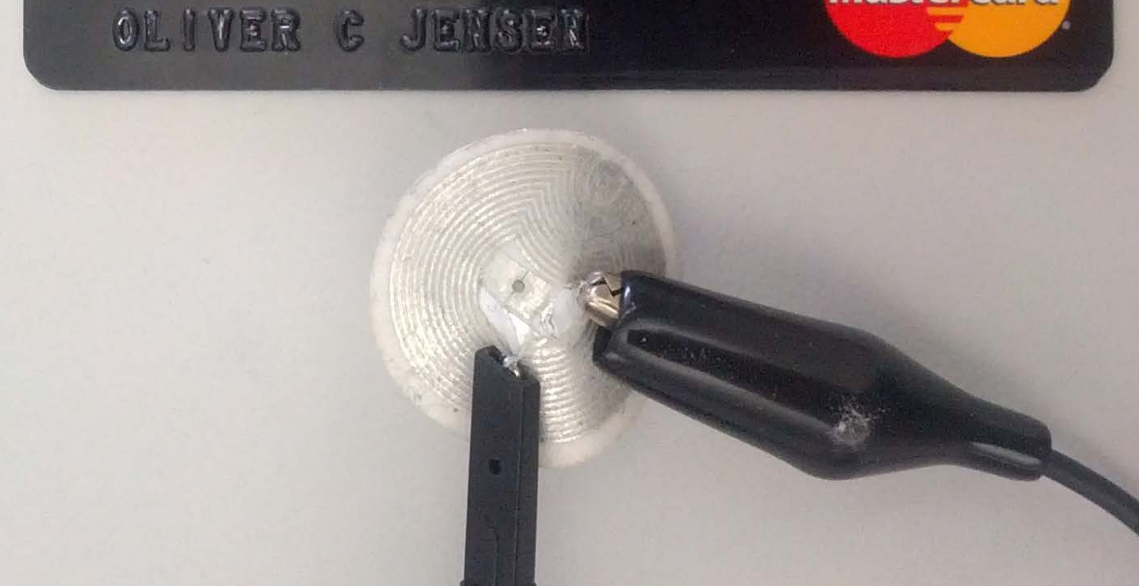
\psfig{file=figures/eavesdroppingAntenna.png,width=3in,natwidth=700,natheight=189}
\caption{Eavesdropping Antenna~\cite{CC2016} \newline(credit card for scale)}
\label{fig:antenna}
\end{figure}
\vspace{2mm}\newline
\noindent\textbf{Skimming:}
In this attack, illustrated in Figure~\ref{fig:skim}, a skimmer gains a victims credit card information, including a single usable iCVV, by masquerading as a point-of-sale. After the skimmer has captured this data, it can replay the credit card information to a genuine point-of-sale to perform an illegitimate purchase on behalf of the victim.

Surprisingly, this attack can be carried out by simply installing an Android application called \textit{NFCProxy}.\footnote{\textit{NFCProxy} was presented at DefCon 20 and can be downloaded at: https://sourceforge.net/projects/nfcproxy/~\cite{CC2016}}
Using \textit{NFCProxy}, any NFC enabled Android device can skim information from a contactless credit card and make a single purchase. To make subsequent purchases, the attack must be repeated to obtain a new iCVVs.
\begin{figure}
\centering
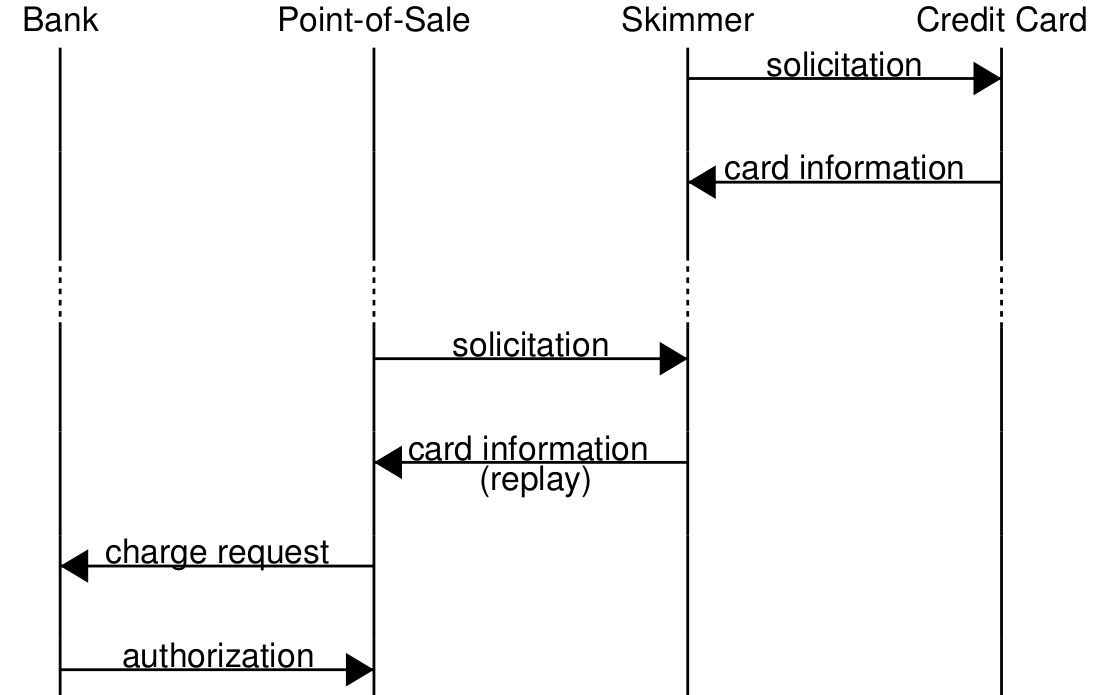
\psfig{file=figures/skim.png,width=3in,natwidth=700,natheight=189}
\caption{Skimming~\cite{CC2016}}
\label{fig:skim}
\end{figure} 
\vspace{2mm}\newline
\noindent\textbf{Relay Attacks:}
The relay attack is similar to the skimming attack, but it does not rely on a single device to skim and replay card data. Instead, two entities work in concert by sharing information over an alternative communication channel, such as wireless LAN.
\vspace{2mm}\newline
\noindent\textbf{Compromised Point-of-Sale:}
This attack points out that since point-of-sale devices learn enough information to allow multiple charges, the point-of-sale is a natural target. If a point-of-sale is compromised, transaction becomes accessible to malicious parties. Jensen, Gouda, and Qiu list several merchants that have recently had their point-of-sale systems compromised including Target, Home Depot, and SuperValu stores.

\subsection{Proposed Secure Credit Card Protocol}
To address these security concerns, Jensen, Gouda, and Qiu have proposed a secure protocol shares the same four phases as the current credit card protocol (Figure~\ref{fig:currentCC}) but with several variations that will be described and illustrated using the Figure~\ref{fig:secureCC}. 

The solicitation phase now includes a random challenge (\textbf{ch}) that will be used by the credit card when building its response. After receiving some basic information and the challenge, the credit card responds by sending the card information in three distinct pieces:
\begin{itemize}
  \item \textbf{A}: \textbf{\textit{UUID}}, a Universally Unique Identifier that to identify the credit card. The UUID is static.
  \item \textbf{B}: \textit{\textbf{H(info, ch, iCVV})} is used to authenticate the card's identity. Notice that the sensitive info, including the card number and expiration date, will not be transmitted in plain text. The details of the hash-like function H are described below.
  \item \textbf{C}: \textbf{\textit{bank name}} is used to route the charge request.
  \end{itemize}
Upon receiving all three parts of the card information, the point-of-sale simply forwards the UUID (\textit{A}) and the authentication (\textit{B}) to the bank (\textit{C}) learning nothing about the actual card data. The challenge (\textit{ch}) is also sent the bank will have all of the pieces necessary to generate the authentication value and check for validity by matching it to (\textit{B}). The bank will also receive the charge amount (\textit{\$}). 

Finally, the bank uses the \textit{UUID} to look up official card data. Then the bank uses  the H function with its own copy of the customer information and the challenge (\textit{ch}) to create \textit{B\begin{tiny}bank\end{tiny}}. If \textit{B\begin{tiny}bank\end{tiny}} = \textit{B}, then the bank considers the card data valid and authorizes the charge.
\vspace{2mm}\newline
\noindent\textbf{Requirements of function H:} So long as \textit{B}, the value returned from the H function, is indistinguishable from random, no sensitive information can be learned from an eavesdropping attack. Also, when a skimming or relay attacker collects \textit{ch} and \textit{B} and attempts to replay the card information, it must not be able to calculate the new value \textit{B$'$} when given the new challenge \textit{ch$'$}.

\todo[inline]{Not sure how to go about describing the H function. Also, I'm already at about 2 pages with just this source... How can I fit this in in a reasonable way? I have already spent way to much room describing protocols and attacks and I still need to fit in two more source summaries + more background + conclusion.}

\begin{figure}
\centering
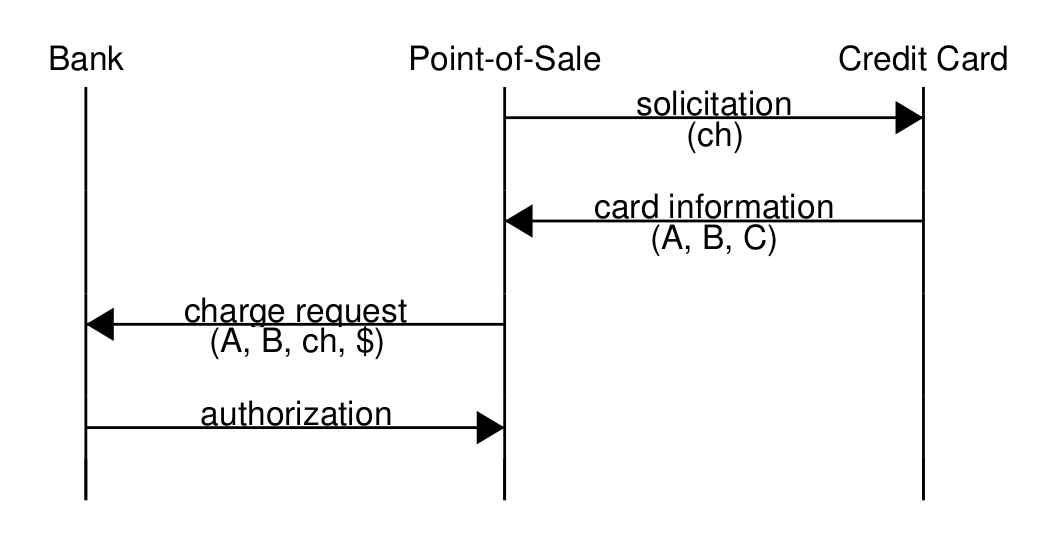
\psfig{file=figures/secureCC.png,width=3in,natwidth=700,natheight=189}
\caption{Purposed Credit Card Protocol~\cite{CC2016}}
\label{fig:secureCC}
\end{figure}

%%%%%%%%%%%%%%%%%%%%%%%%%%%%%%%%%%%%%%%%%%%%%%%%%%%%%%%%%%%%%%%%%%%%%
%%%%%%%%%%%%%%%%%%%%%%%%%%%%%%%%%%%%%%%%%%%%%%%%%%%%%%%%%%%%%%%%%%%%%
%%%%%%%%%%%%%%%%%%%%%%%%%%%%%%%%%%%%%%%%%%%%%%%%%%%%%%%%%%%%%%%%%%%%%
%%%%%%%%%%%%%%%%%%%%%%%%%%%%%%%%%%%%%%%%%%%%%%%%%%%%%%%%%%%%%%%%%%%%%


\section{NFC and Mass Transit Ticketing}
\label{sec:mobile}

Mass transit systems have widely adopted contactless NFC cards for identity verification and ticketing. Three Nokia researchers, Tamrakar, Ekberg, and Asokan, have punished a paper investigating the use of NFC-enabled mobile phones for this application. In their paper, they first describe the the pieces involved in building a complete identity-verification ticketing architecture. Then, three implementations of mobile ticketing, each balancing security and transaction time in a unique way, are introduced, prototyped, and critiqued.\cite{Ticket2011}

\subsection{Ticketing Architecture}

\begin{figure}
\centering
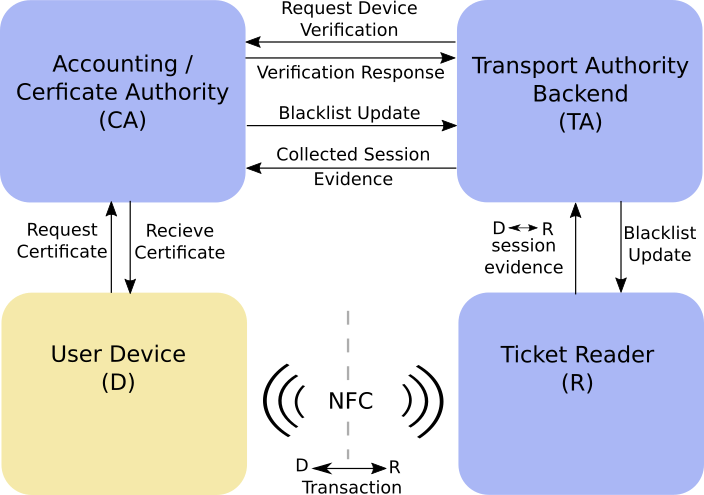
\psfig{file=figures/ticketingArch.png,width=3in,natwidth=700,natheight=189}
\caption{Ticketing Architecture~\cite{Ticket2011}}
\label{fig:secureCC}
\end{figure}


%%%%%%%%%%%%%%%%%%%%%%%%%%%%%%%%%%%%%%%%%%%%%%%%%%%%%%%%%%%%%%%%%%%%%
%%%%%%%%%%%%%%%%%%%%%%%%%%%%%%%%%%%%%%%%%%%%%%%%%%%%%%%%%%%%%%%%%%%%%
%%%%%%%%%%%%%%%%%%%%%%%%%%%%%%%%%%%%%%%%%%%%%%%%%%%%%%%%%%%%%%%%%%%%%
%%%%%%%%%%%%%%%%%%%%%%%%%%%%%%%%%%%%%%%%%%%%%%%%%%%%%%%%%%%%%%%%%%%%%
\section{EnGarde: A Physical Approach to NFC Security}
\label{sec:enGarde}

\begin{figure}
\centering
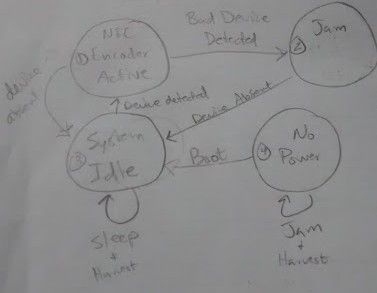
\psfig{file=figures/states.jpg,width=3in,natwidth=700,natheight=189}
\caption{Simplified EnGarde\cite{Gum2013} state digram}
\label{fig:states}
\end{figure}

Commercial payment systems such as Apple Pay and Android Pay are bringing NFC to our phones, which could introduce security risks in both payment and non-payment applications of NFC. A programmable, hardware-based firewall may be a viable way to defend against more general threats as new applications and attacks are developed. EnGarde is designed to be an extremely power efficient, semi-permanent attachment for everyday mobile phones. Such a device-independent security method, a metaphorical tin foil hat, could offer flexibly against current and evolving attacks on NFC enabled devices.~\cite{Gum2013}

Our goal is to give an overview of the EnGarde security system prototyped by Gummeson et al. Figure \ref{fig:states}, is used as a roadmap for our summary of EnGarde and its components.

\subsection{No Power Mode}

EnGarde is device-independent and is thus not powered directly from the battery contained within the cellphone it is mounted to. Instead, EnGarde contains its own dedicated battery that is charged exclusively by electricity induced into its NFC antenna.\footnote{Power scavenging methods are addressed in great detail in the primary source, but for the this paper, we will not focus how harvesting adequate power from the cellphone works in practice.} 
As a result of being independently powered, EnGarde can run on battery and encounter a no-power state. Thus, EnGarde was intentionally designed to fail safe. When EnGarde is in the no power state, it cannot do anything until an NFC signal is detected from either the host phone or an external device. At this point, EnGarde collects power from the NFC signal while simultaneously jamming the ongoing communication. Once enough power is collected, control is handed to the microcontroller.

\subsection{System Idle Mode}
In the system idle state, the microcontroller is running and the EnGarde device simply manages power and waits for an NFC device to move into its vicinity. When an NFC signal is detected, the NFC decoder is activated.

\subsection{NFC Decoder Active Mode}
In this state, we discuss EnGarde's ability to use discretion to block or allow each NFC communication. To do this EnGarde actively scans each transmission from the nearby NFC device in order to determines the other party's intent. EnGarde is designed to offer real-time protection against malicious attacks from all NFC modes:
\vspace{2mm}\newline
\noindent\textbf{Malicious Tags}: NFC tags can be handy for storing data or URLs in real world applications such as content rich maps or posters. However, such a tag may contain undesirable content, such as a URL to a malicious website. 
\vspace{2mm}\newline
\noindent\textbf{Malicious Peer}: Since NFC supports file transfers from peers, an NFC phone is ultimately vulnerable to whatever is sent from the peer.
\vspace{2mm}\newline
\noindent\textbf{Malicious Reader}: Unauthorized readers may attempt to interact with a phone when it is in tag-emulation mode. The phone's location would be known each time a tag ID is read, which effectively enables a form of tracking on that mobile device. Alternatively, a malicious reader could potentially compromise the phone owner's financial data.
\vspace{2mm}\newline
\noindent\textbf{Malicious Software Installations}: The phone owner may inadvertently install malicious software with permission to broadcast via NFC. EnGarde should be able to prevent undesired information sharing over the NFC interface.
\vspace{2mm}\newline
To handle malicious communication, EnGarde scans each message and uses a set of blocking rules to determine if that message should be allowed. The EnGarde is versatile in that current and future undesirable transmissions can be addressed by updating the blocking rules and blacklist.

\subsection{Jam Mode}
When in this mode, EnGarde's goal is to prevent malicious incoming and outgoing communication over NFC. To do this, EnGarde depends on two jamming primitives:
\vspace{2mm}\newline
\noindent\textbf{Reflective Jamming:} This defense mechanism is effective against attacks from low-powered tags containing items such as malicious URLs. It works by simply generating a weak signal on the same frequency that the tag is broadcasting to. Since EnGarde is mounted on the back of the owner's phone, EnGarde's signal will be stronger and will effectively block the malicious tag's messages. In additional, the electricity being used to power the tag will also be used to power EnGarde's active defense.
\vspace{2mm}\newline
\noindent\textbf{Pulse Jamming:} If the phone is being attacked by a powered reader or peer device, a much stronger defense, namely generating a competing active transmission, is required to protect the mobile phone. A continuous active transmission would demand far more power then EnGarde could scavenge. Gummeson et al's response to is to simply corrupt incoming communication in this case. To corrupt the incoming signal, EnGarde needs to generate a pulse lasting only about 20 microseconds. This brief duration is long enough to corrupt two bits of data, even at the slowest NFC transmission rate.

There is, however, a drawback to the pulse jamming method; a sufficiently high-powered reader could generate a strong enough signal to nullify EnGarde's attempts to corrupt the incoming data. Yet, Gummeson et al counter that an active attack from a high powered reader could be mitigated by using the \textit{reflective jamming} method during the offending reader's discovery protocol. If a connection with a high-powered reader is never established, then EnGarde would not have to use the pulse jamming mechanism against a high-powered reader.

\subsection{Experimental Evaluation of EnGarde}
\noindent\textbf{Jamming:} Both of EnGarde's jamming primitives are surprisingly effective. In fact, when Gummeson et al evaluated their device, they found that reflective jamming worked flawlessly against four tags that they tested against. Additionally, they tested the pulse jamming method with general purpose NFC reader and found that EnGarde was able to block 100\% of the responses.
\vspace{2mm}\newline
\noindent\textbf{Decoding:} 
When trying to read tags, one of which contained a blacklisted URL, they found that EnGarde blocked the malicious URL and allowed the benign URL every time.
\vspace{2mm}\newline
It appears that EnGarde was extraordinarily successful given the official results.

\section{Conclusions}
\label{sec:conclusions}

It was cool. Tin foil hats for all.

\section*{Acknowledgments}
\label{sec:acknowledgments}


It is common (but by no means necessary) for students to thank
their advisor, and possibly other faculty, friends, and family who provided
useful feedback on the paper as it was being written. -> Nic, Elena, KK, Kevin

% The following two commands are all you need in the
% initial runs of your .tex file to
% produce the bibliography for the citations in your paper.
\bibliographystyle{abbrv}
% sample_paper.bib is the name of the BibTex file containing the
% bibliography entries. Note that you *don't* include the .bib ending here.
\bibliography{tomSources}  
% You must have a proper ".bib" file
%  and remember to run:
% latex bibtex latex latex
% to resolve all references
\end{document}
